This section outlines the testbed developed for CloudVR experiments, which leverages the NVIDIA CloudXR architecture to deliver immersive virtual reality experiences over wireless networks. We begin by providing an overview of the CloudVR application framework, followed by a detailed description of the testbed infrastructure and automation components.

\subsection{Testbed Infrastructure}

The testbed is built upon the NVIDIA CloudXR SDK, an \ac{XR} streaming platform that utilizes edge computing and cloud-based GPU acceleration to deliver high-fidelity VR experiences. The CloudXR platform streams OpenVR-based applications from a remote server to XR client devices with limited graphical capabilities, such as the untethered \ac{HMDs} Meta Quest 2 and Meta Quest 3. These devices connect to the server through various network interfaces, including Ethernet, Wi-Fi, or cellular connections.

The CloudXR architecture comprises a server-side driver responsible for streaming audio and video content from XR applications (e.g., SteamVR) to the client device using network protocols like UDP; a client-side software that enables the HMD to receive and render streamed VR content, ensuring low-latency interactions and maintaining high-quality visuals.

The CloudVR testbed, as depicted in Fig. \ref{fig:chap_6:testbed}, facilitates controlled experiments under realistic network conditions. The testbed consists of a server (a machine with an Intel Xeon W2235 CPU @ 3.8GHz, 32 GB of RAM, and an NVIDIA GeForce RTX 3090 Ti GPU) running the CloudXR server software to render and stream VR content; a client (Meta Quest 2 HMD) wirelessly connected to the network and a Wi-Fi \ac{AP} (here a Orange Livebox router).

\begin{figure*}[!ht]
    \centering
    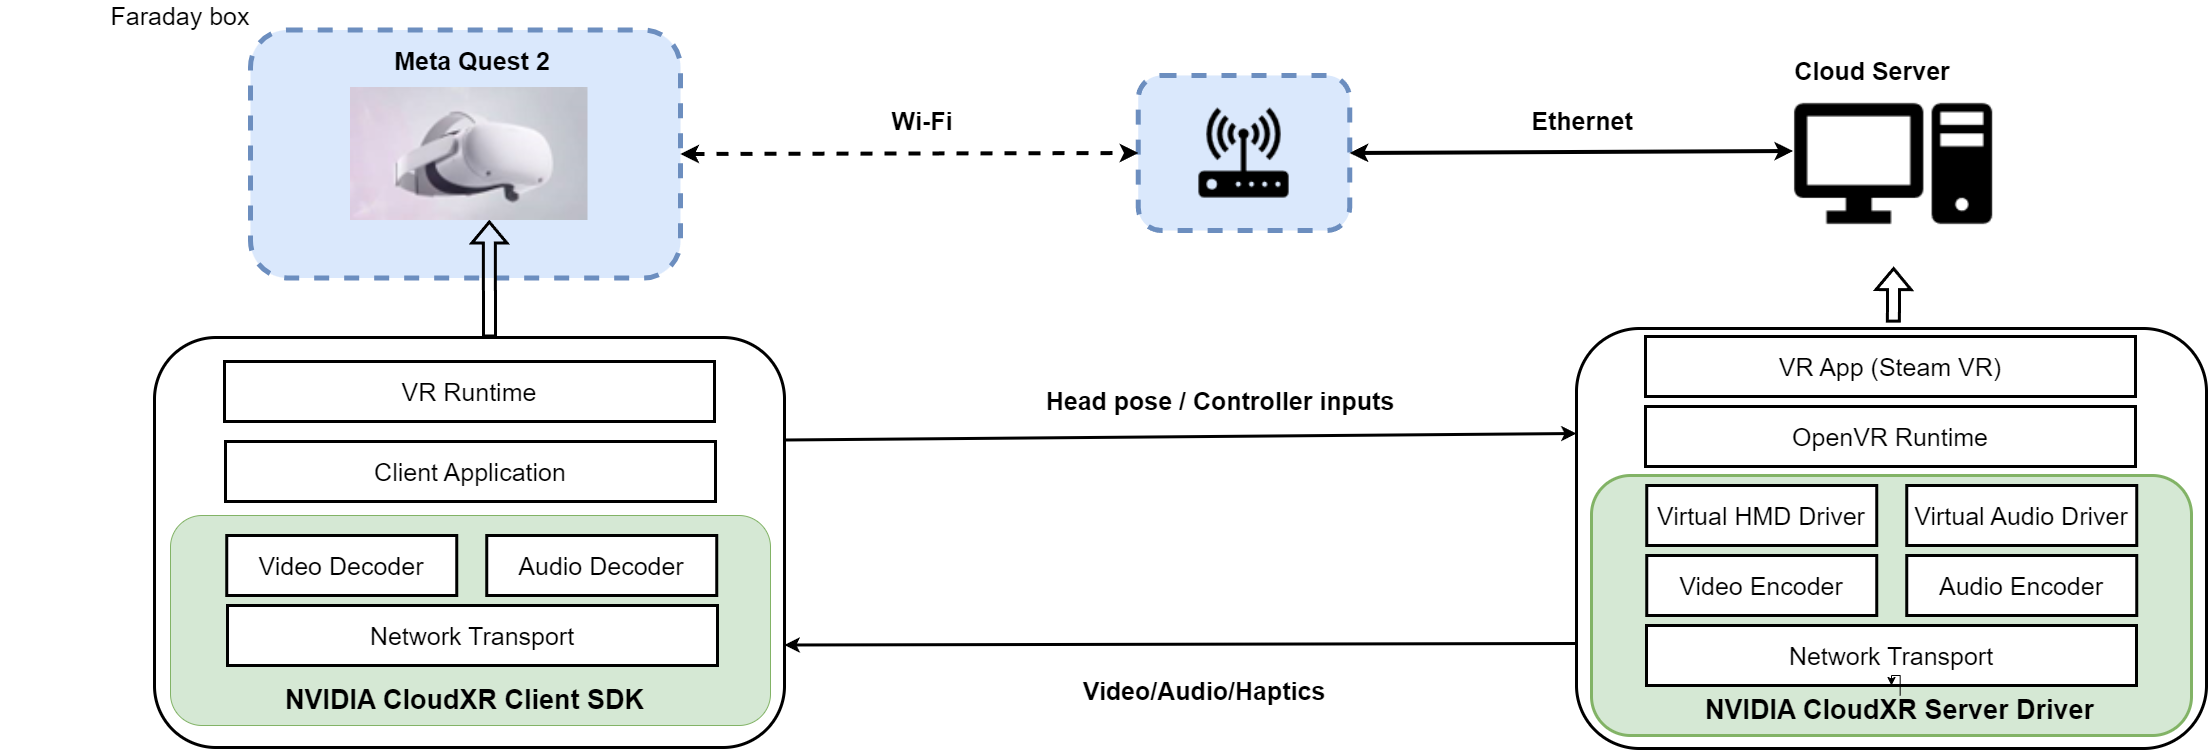
\includegraphics[width=\linewidth]{imgs/chapter_6/cloud_xr_stack.png}
    \caption{Cloud VR testbed}
    \label{fig:chap_6:testbed}
\end{figure*}


%-------------------description of FA testbed (Minqi Nicolas)--------------------

\begin{figure*}[!ht]
    \centering
    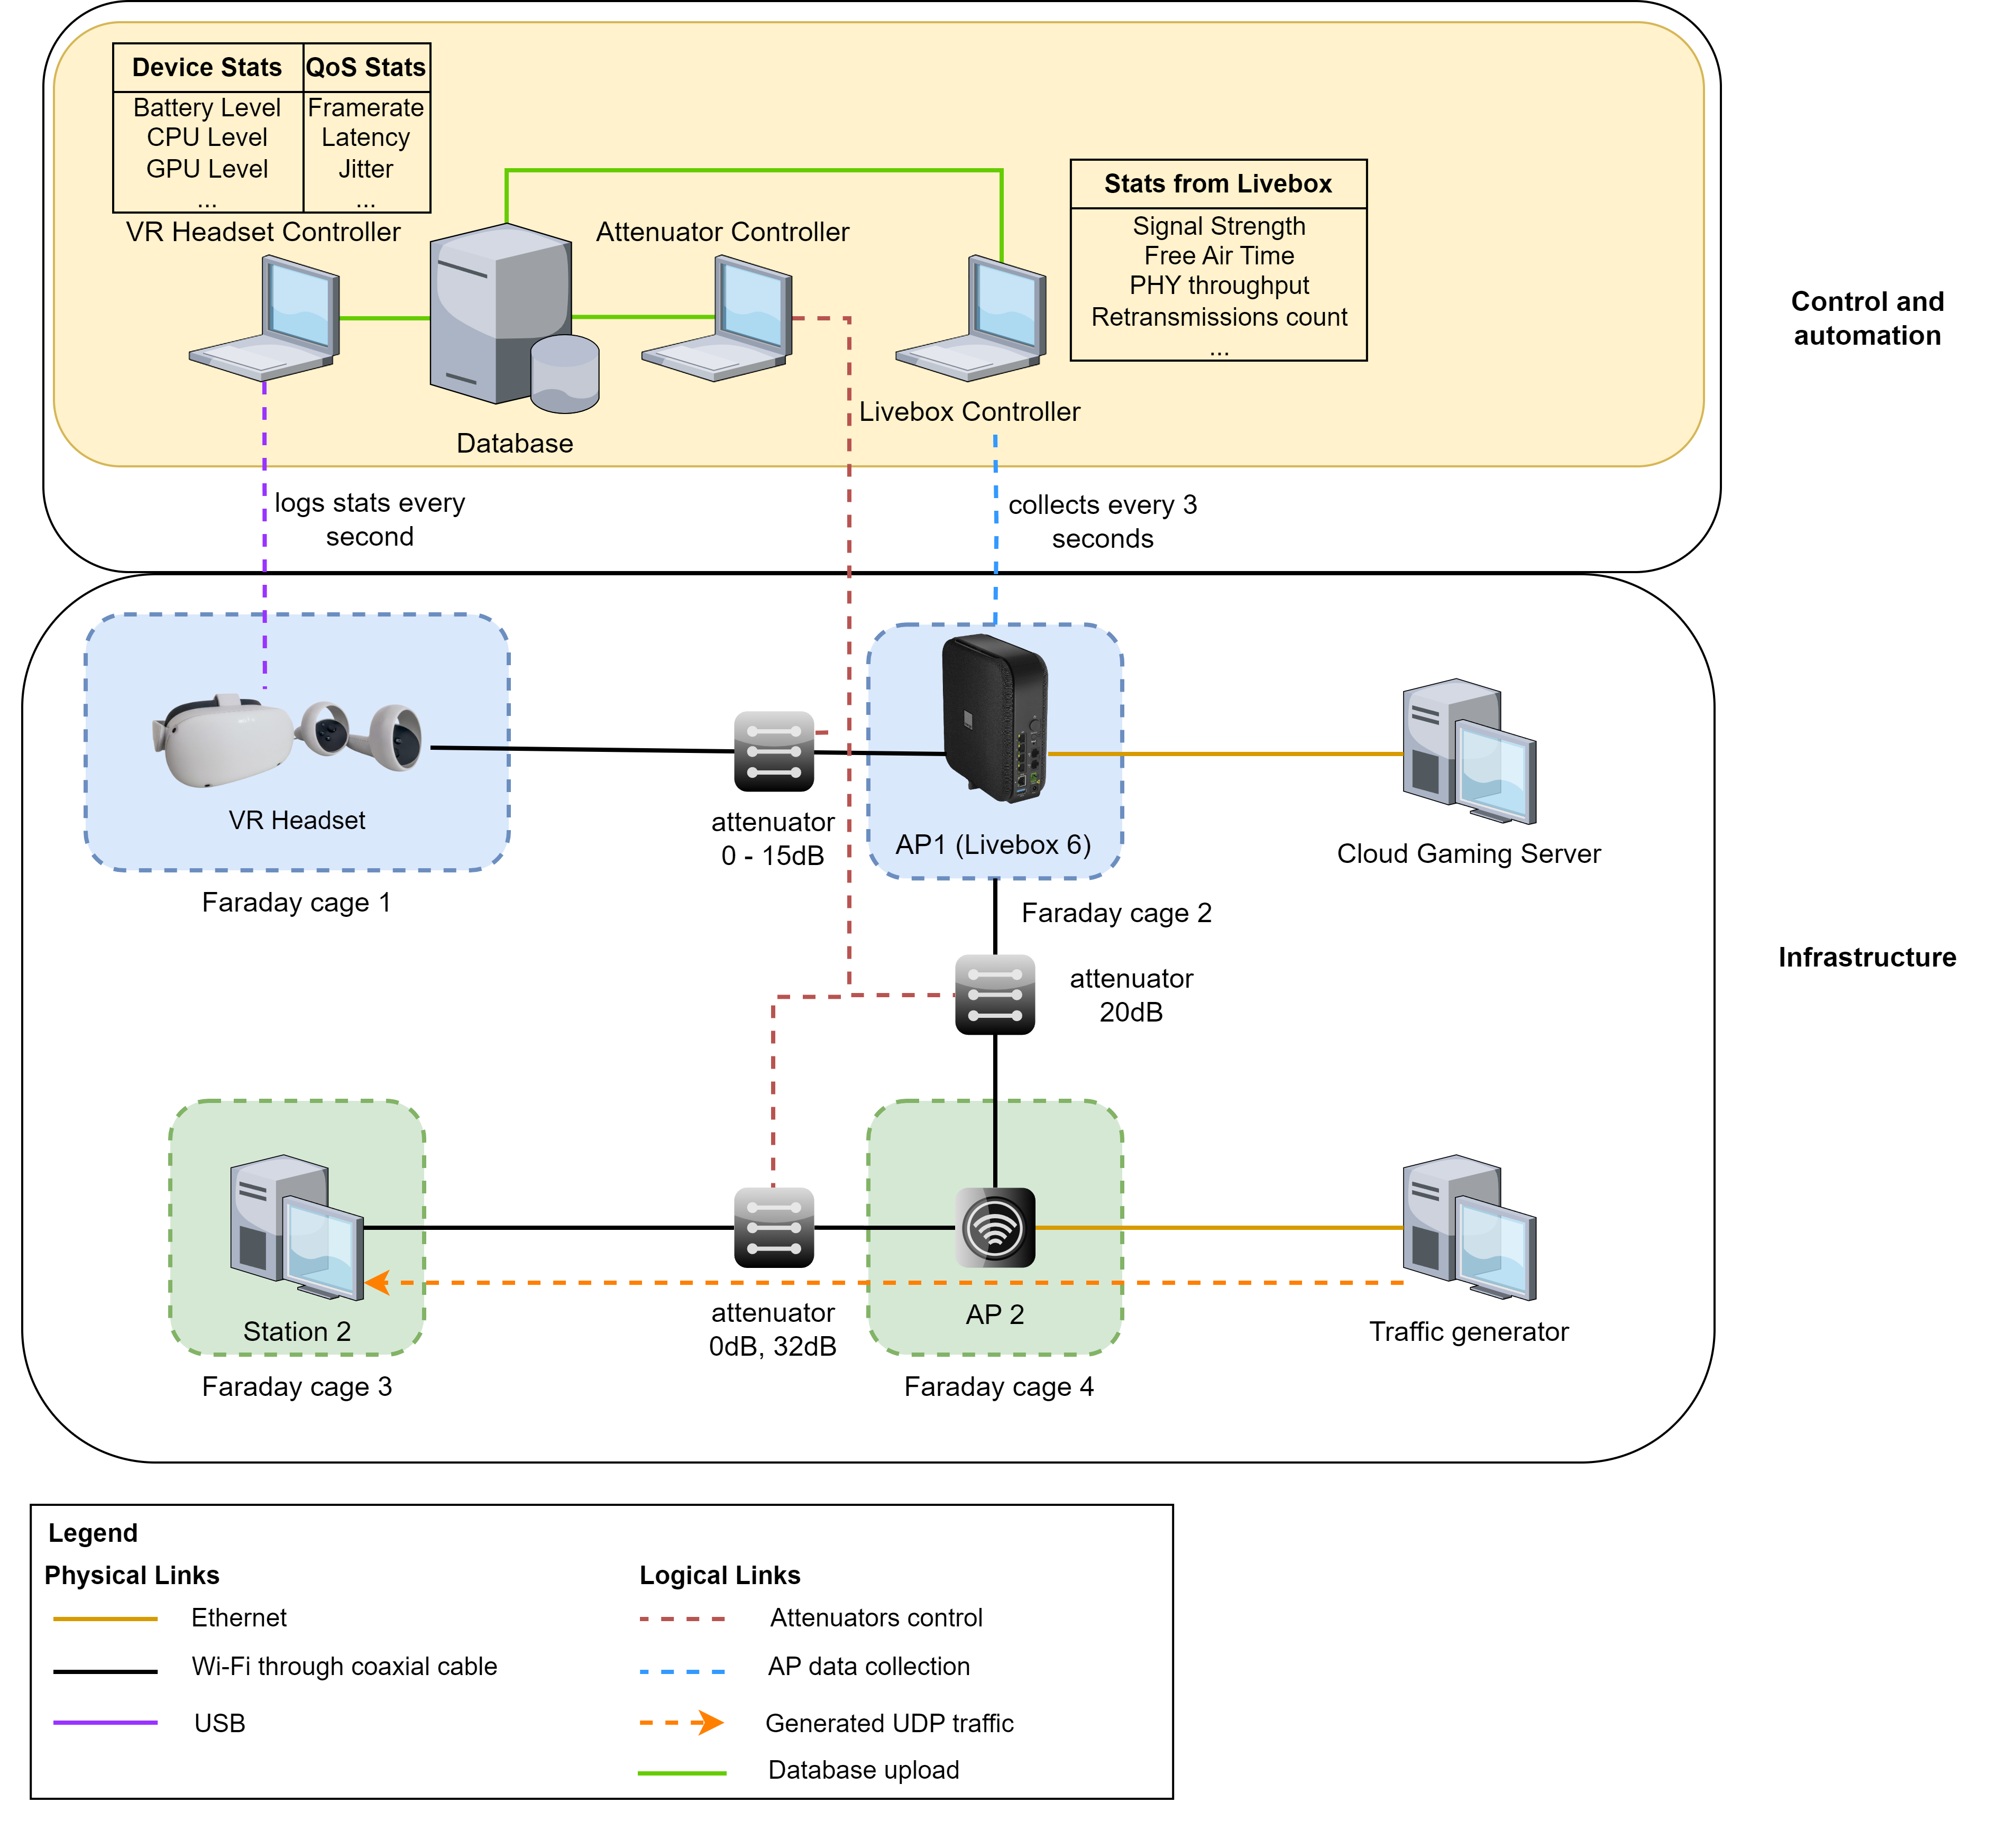
\includegraphics[width=\linewidth]{imgs/chapter_6/WiFi_testbed.png}
    \caption{Wi-Fi testbed for Cloud VR scenarios}
    \label{fig:chap_6:testbed_wifi}
\end{figure*}




\subsection{Wi-Fi Testbed for Controlled Experiments}

We designed a controlled Wi-Fi testbed, illustrated in Fig. \ref{fig:chap_6:testbed_wifi}, to replicate real-world Wi-Fi network impairments that can impact Cloud VR performance, with the goal of detecting these issues through root cause diagnosis.

The testbed consists of two primary layers:
\begin{itemize}
    \item \textbf{Infrastructure layer:} This layer includes up to four Faraday cages used to isolate equipment from external electromagnetic interference. The cages are allocated as follows: one for the VR headset, two for the APs, and one for a station used in interference scenarios. The layer also includes two access points (AP1 and AP2): AP1 is utilized for normal and coverage experiments, while AP2 introduces interference in specific scenarios. The Faraday cages are interconnected using coaxial cables to transmit Wi-Fi signals, and \ac{RF} attenuators \footnote{\url{https://adauratech.com/attenuators/}} are employed to simulate variations in signal strength during experiments. Two servers are part of this setup: the first server (see Fig. \ref{fig:chap_6:testbed}) runs the CloudVR software and is connected to AP1 via Ethernet, while the second server acts as a traffic generator connected to AP2, simulating competing downlink traffic using UDP.

    \item \textbf{Control and Automation layer:} This layer includes a VR PC controller connected to the VR headset via USB, responsible for managing headset settings and collecting performance metrics, such as key performance indicators (KPIs) from OVR Metrics tools\footnote{\url{https://developers.meta.com/horizon/downloads/package/ovr-metrics-tool/}} or quality-of-service (QoS) statistics from CloudXR. The controller also automates game sessions using the Meta Quest Autodriver\footnote{\url{https://developers.meta.com/horizon/documentation/unity/ts-autodriver}}. Additionally, this layer features an attenuator controller that configures and manages RF attenuators via APIs, enabling automated signal attenuation adjustments through FastAPI \footnote{\url{https://fastapi.tiangolo.com/}}. Furthermore, the Livebox controller manages the Livebox via Telnet to collect Wi-Fi KPIs every 3 seconds. A local ELK Stack \footnote{\url{https://www.elastic.co/fr/elastic-stack}} database aggregates data from all controllers for post-experiment analysis.

\end{itemize}

\subsection{Experimental Scenarios}

We collect Cloud VR data across several controlled scenarios using the Beat Saber game as a benchmark. These scenarios were executed on both the 2.4 GHz and 5 GHz frequency bands, as detailed below:
\begin{itemize}
    \item Normal scenarios: CloudVR sessions are conducted under ideal conditions, with no network impairments. The VR headset is placed in an optimal coverage area and connected to AP1 for each frequency band. A total of five 300-second sessions were performed for each of the frequency bands.
    \item Coverage scenarios: To simulate variations in signal strength, RF attenuators are used to modify the \ac{RSSI} during VR sessions. The following RSSI values were tested for 2.4 GHz: \{-55 dB, -60 dB, -65 dB\} and for 5 GHz: \{-80 dB, -85 dB, -90 dB\}. Each RSSI configuration is tested in three sessions, each lasting 100 seconds.
    \item Interference scenarios: Interference is introduced by a neighboring station connected to AP2, which operated on the same frequency and bandwidth as AP1. The interference is simulated by limiting the transmission opportunities (txops) available on AP1 after starting the game. The following interference levels were tested for 2.4 GHz: 85\% and 90\% of txops are occupied by AP2 and for 5 GHz: 89\%, 90\%, and 91\% of txops are occupied by AP2. Each interference configuration is tested in three sessions, with each session lasting 100 seconds.
\end{itemize}


This testbed design ensures a highly controlled environment for conducting CloudVR experiments. By leveraging Faraday cages, we eliminate uncontrolled external radio interference. The deployment of local servers minimizes external network variability, and automation tools enable seamless execution of experiments with precise configuration and data collection.



